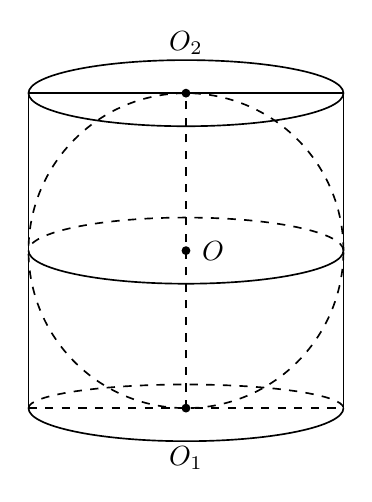
\begin{tikzpicture}[line width=0.6pt, font=\normalsize]
\tikzset{hid/.style={dashed}, lbl/.style={font=\normalsize, fill=white, inner sep=1.5pt}}
\def\rx{2.0} \def\ry{0.42} \def\h{2.0}
% cylinder walls
\draw (-\rx,-\h)--(-\rx,\h) (\rx,-\h)--(\rx,\h);
% top rim + diameter
\draw (0,\h) ellipse (\rx cm and \ry cm);
\draw (-\rx,\h)--(\rx,\h);
% bottom rim front solid / diameter dashed
\draw (-\rx,-\h) arc (180:360:\rx cm and \ry cm);
\draw[hid] (-\rx,-\h)--(\rx,-\h);
\draw[hid] (-\rx,-\h) arc (180:0:\rx cm and 0.30cm);
\draw[hid] (0,0) circle (2cm);
% equator of sphere: front solid, back dashed
\draw (-\rx,0) arc (180:360:\rx cm and \ry cm);
\draw[hid] (\rx,0) arc (0:180:\rx cm and \ry cm);
% mid dashed ellipse (sphere back latitude) to match original
% axis
\draw[hid] (0,-\h)--(0,\h);
\fill (0,0) circle (1.6pt); \fill (0,\h) circle (1.6pt); \fill (0,-\h) circle (1.6pt);
\node[lbl, right=4pt] at (0,0) {$O$};
\node[lbl, below=4pt,xshift=0.00bp,yshift=-8.00bp] at (0,-\h) {$O_{1}$};
\node[lbl, above=4pt,xshift=0.00bp,yshift=8.00bp] at (0,\h) {$O_{2}$};
\end{tikzpicture}
